\documentclass[border=10pt]{standalone}
\usepackage{pgfplots}
\pgfplotsset{compat=1.18}
\begin{document}
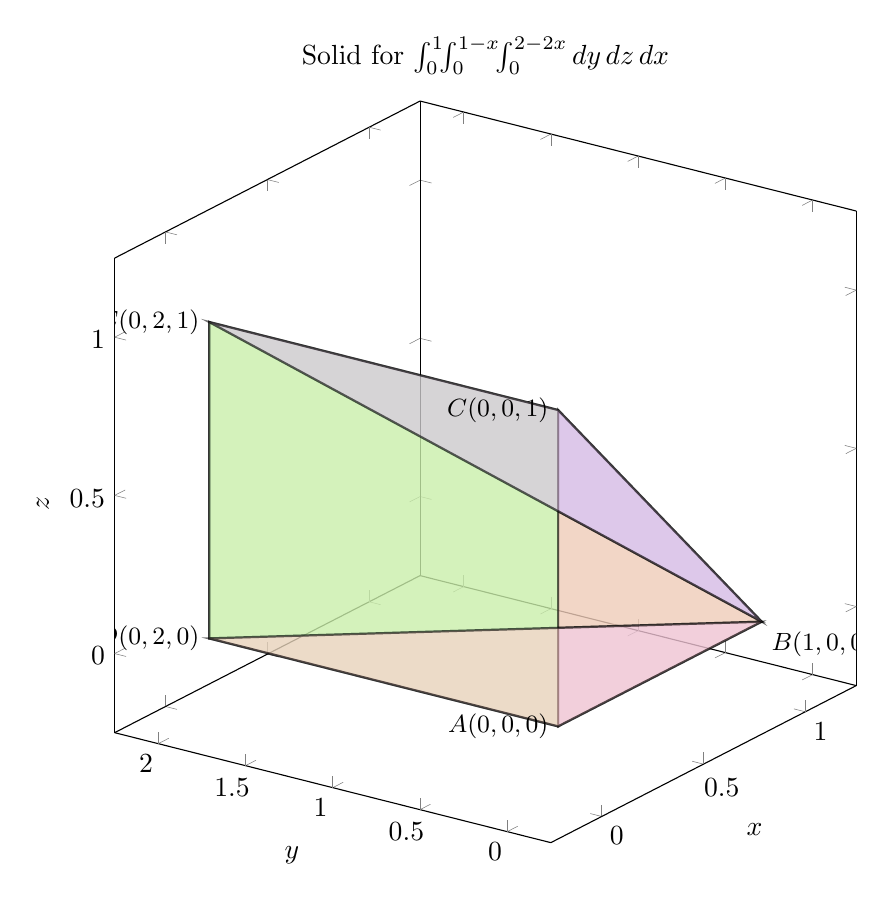
\begin{tikzpicture}
\begin{axis}[
    view={-55}{22},
    xlabel={$x$}, ylabel={$y$}, zlabel={$z$},
    xmin=-0.25, xmax=1.25, ymin=-0.25, ymax=2.25, zmin=-0.25, zmax=1.25,
    width=11cm, height=11cm,
    title={Solid for $\int_0^1\!\!\int_0^{1-x}\!\!\int_0^{2-2x} dy\,dz\,dx$},
]

% Bottom (y=0): triangle (0,0,0)-(1,0,0)-(0,0,1)
\addplot3[fill=blue!20, draw=black, thick, opacity=0.55] coordinates {
    (0,0,0) (1,0,0) (0,0,1) (0,0,0)} -- cycle;

% Top (y=2-2x): triangle (0,2,0)-(1,0,0)-(0,2,1)
\addplot3[fill=orange!40, draw=black, thick, opacity=0.55] coordinates {
    (0,2,0) (1,0,0) (0,2,1) (0,2,0)} -- cycle;

% Back (x=0): rectangle (0,0,0)-(0,2,0)-(0,2,1)-(0,0,1)
\addplot3[fill=green!30, draw=black, thick, opacity=0.55] coordinates {
    (0,0,0) (0,2,0) (0,2,1) (0,0,1) (0,0,0)} -- cycle;

% Front-left (z=0): triangle (0,0,0)-(1,0,0)-(0,2,0)
\addplot3[fill=red!25, draw=black, thick, opacity=0.55] coordinates {
    (0,0,0) (1,0,0) (0,2,0) (0,0,0)} -- cycle;

% Slanted (x+z=1): triangle (0,0,1)-(0,2,1)-(1,0,0)
\addplot3[fill=violet!30, draw=black, thick, opacity=0.55] coordinates {
    (0,0,1) (0,2,1) (1,0,0) (0,0,1)} -- cycle;

% Vertex labels
\node[anchor=east]      at (axis cs:0,0,0)    {\small $A(0,0,0)$};
\node[anchor=north west]at (axis cs:1,0,0)    {\small $B(1,0,0)$};
\node[anchor=east]      at (axis cs:0,0,1)    {\small $C(0,0,1)$};
\node[anchor=east]      at (axis cs:0,2,0)    {\small $D(0,2,0)$};
\node[anchor=east]      at (axis cs:0,2,1)    {\small $E(0,2,1)$};

\end{axis}
\end{tikzpicture}
\end{document}
